% THIS IS AN EXAMPLE DOCUMENT FOR VLDB 2012
% based on ACM SIGPROC-SP.TEX VERSION 2.7
% Modified by  Gerald Weber <gerald@cs.auckland.ac.nz>
% Removed the requirement to include *bbl file in here. (AhmetSacan, Sep2012)
% Fixed the equation on page 3 to prevent line overflow. (AhmetSacan, Sep2012)
\listfiles
\documentclass{sig-alternate}
\usepackage{graphicx}
\usepackage{color}
\usepackage{balance}  % for  \balance command ON LAST PAGE  (only there!)
\usepackage{times}
\usepackage{url}
\usepackage{algorithm}
\usepackage[noend]{algorithmic}
\usepackage{subfigure}
\usepackage{xspace}
\usepackage[noend]{algorithmic}
\usepackage{enumerate}
\usepackage{multirow}
\usepackage{epstopdf}
\usepackage{cleveref}
\usepackage[font={small,it}]{caption}

\newcommand{\squishlist}{
   \begin{list}{$\bullet$}
    {
      \setlength{\itemsep}{0pt}
      \setlength{\parsep}{3pt}
      \setlength{\topsep}{3pt}
      \setlength{\partopsep}{0pt}
      \setlength{\leftmargin}{1.5em}
      \setlength{\labelwidth}{1em}
      \setlength{\labelsep}{0.5em} } }

\newcommand{\squishend}{
    \end{list}  }

\renewcommand*\ttdefault{cmvtt}

\makeatletter
\def\@copyrightspace{\relax}
\makeatother


\newcommand{\argmax}{\operatornamewithlimits{arg\ max}}

\newcommand{\eat}[1]{}
\newcommand{\todo}[1]{\textcolor{red}{{TODO: #1}}}
\newcommand{\add}[1]{\textcolor{red}{{ADD: #1}}}
\newcommand{\note}[1]{\textcolor{blue}{{#1}}}
\newcommand{\agp}[1]{\textcolor{blue}{{Aditya: #1}}}
\newcommand{\stitle}[1]{\vspace{0.5em}\noindent\textbf{#1}}


\newtheorem{definition}{Definition}
\newtheorem{example}{Example}
\newtheorem{theorem}{Theorem}
\newtheorem{lemma}{Lemma}
\newtheorem{problem}{Problem}
\newtheorem{reduction}{Reduction}
\newcommand{\domain}{\mathcal{D}}
\newcommand{\attributes}{\mathcal{A}_D}
\newcommand{\hierarchy}{\mathcal{H}_D}
\newcommand{\attrhierarchy}{\mathcal{H}_A}
\newcommand{\workers}{\mathcal{W}}
\newcommand{\uentities}{\mathcal{E}}
\newcommand{\queryvector}{{\bf Q_S}}



\begin{document}

% ****************** TITLE ****************************************

\title{CrowdGather: Entity Extraction over Structured Domains}

\numberofauthors{3} 

\author{
	\alignauthor Theodoros Rekatsinas\\
            \affaddr{University of Maryland, College Park} 
                \email{thodrek@cs.umd.edu}
            \alignauthor Amol Deshpande\\
            \affaddr{University of Maryland, College Park} 
                \email{amol@cs.umd.edu}
            \alignauthor Aditya Parameswaran \\
            \affaddr{University of Illinois, Urbana-Champaign} 
                \email{adityagp@illinois.edu}
}

\maketitle

\begin{abstract}
Crowdsourced entity extraction is often used to acquire data for many applications, including recommendation systems, 
construction of aggregated listings and directories, and knowledge base construction. Current solutions focus on entity extraction using a single query, e.g., only using ``give me another restaurant", when assembling a list of all restaurants. Due to the cost of human labor, just focusing on a single query limits the practical applicability of these solutions.

In this paper, we leverage {\em structured entity domains}, i.e., domains that can be fully described by a collection of attributes, each potentially displaying hierarchical structure. Given such an entity domain, we enable a richer space of queries, e.g., ``give me another Moroccan restaurant in Manhattan that does takeout". Naturally, enabling a richer space of queries comes with a host of issues, especially since many queries return empty answers. We develop new statistical tools that enable us to reason about the gain of issuing {\em additional queries} given little to no information, and show how we can exploit the overlaps across the results of queries for different points of the data domain to obtain accurate estimates of the gain. We cast the problem of {\em budgeted entity extraction} over large domains as an adaptive optimization problem that seeks to maximize the number of extracted entities, while minimizing the overall extraction costs. We evaluate our techniques with experiments on both synthetic and real-world datasets, demonstrating a yield of up to 4X over competing approaches for the same budget.
\end{abstract}

%!TEX root = ../crowd_hierarchies_v.1.3.tex

% THIS IS AN EXAMPLE DOCUMENT FOR VLDB 2012
% based on ACM SIGPROC-SP.TEX VERSION 2.7
% Modified by  Gerald Weber <gerald@cs.auckland.ac.nz>
% Removed the requirement to include *bbl file in here. (AhmetSacan, Sep2012)
% Fixed the equation on page 3 to prevent line overflow. (AhmetSacan, Sep2012)


\section{Introduction}
\label{sec:intro}
Combining human computation with traditional computation, commonly referred to as {\em crowdsourcing}, has been recently proven beneficial in extracting knowledge and acquiring data for many application domains, including recommendation systems~\cite{amsterdamer:2014}, knowledge base completion~\cite{kondredi:2014}, entity extraction and structured data collection~\cite{park:2014,trushkowsky:2013}. In fact, extracting information, and entities in particular, from the crowd has been shown to provide access to more fine-grained information that may belong to the long tail of the web or even be completely unavailable on the web~\cite{franklin:2011, Parameswaran:2012, west:2014}.

A fundamental challenge in crowdsourced entity extraction is reasoning about the completeness of the extracted information. More precisely, given a task that seeks to extract entities from a specific domain by asking human workers, e.g., ``extract all restaurants in New York", it is not easy to judge if we have extracted all entities (in this case restaurants). This is because we are in an ``open world"~\cite{franklin:2011} scenario. 

Recent work~\cite{trushkowsky:2013} has considered the problem of crowdsourced entity extraction using a single type of {\em query} that is asked to humans; for our restaurant case, the query will be ``give me another restaurant in New York''. That paper determines how many times this query must be asked to different human workers before we are sure we have extracted all restaurants in New York. However, given the monetary cost inherent in leveraging crowdsourcing, it is easy to see that just using this query repeatedly will not be practical for real-world applications, for two coupled reasons: (a) {\em wasted cost:} we will keep receiving the most popular restaurants and will have to issue many additional queries before receiving new or unseen restaurants, thus, increasing the cost (b) {\em lack of coverage:}  beyond a point all the restaurants we get will already be present in our set of extracted entities --- thus, for the less popular restaurants, we may never end up receiving them at all.

In this paper, our goal is to {\em make crowdsourced entity extraction practical}. To do so, we leverage a structured entity domain, i.e., a domain that can be fully described by a collection of attributes, each potentially displaying hierarchical structure. For example, in our restaurant case, we could have one attribute about location, one about cuisine, and one about whether the restaurant does takeout. Often the structure of domains in practical applications is already known by design. We can then leverage this structure to use a much richer space of queries asked to human workers, considering all combinations of values for each of these attributes, e.g., ``give me another Moroccan restaurant in Manhattan, New York, that does takeout".  In this manner, we can leverage these {\em specific, targeted queries} to extract not-so popular entities with attribute values set to specific ones, e.g., in this case, cuisine is ``Moroccan", location is ``Manhattan", and takeout is ``Yes".

If we view the structured data domain as a \emph{partially ordered set} (poset), then each query can be mapped to a node in the graph describing its topology. Thus, our goal is to traverse the graph corresponding to the input poset by issuing queries corresponding to various nodes, often multiple times at each node. However, the poset describing the domain can be often large, leading to many additional challenges in deciding which queries to issue at any node: (a) {\em Sparsity:} Many of the nodes in the poset are likely to be empty, i.e., the queries corresponding to those nodes are likely to not have any answers; avoiding asking queries corresponding to these nodes is essential to keep monetary cost low. (b) {\em Interrelationships:} Many of the nodes in the poset are ``coupled'' with one another; for example, the results from a few queries corresponding to ``give me another Moroccan restaurant in Manhattan, New York'' can inform whether issuing queries corresponding to ``give me another Moroccan restaurant in Manhattan, New York, that does takeout'' is useful or not. We elaborate more on these challenges in \Cref{sec:challenges} using examples from a real-world scenario.

Previously proposed techniques~\cite{trushkowsky:2013} do not directly apply to the scenario where we are traversing a poset corresponding to this structured data domain, and new techniques are needed. The main limitation of the aforementioned techniques is that they focus on estimating the completeness of a specific query and are agnostic to cost. As a consequence they do not address the problem of deciding which additional queries are \emph{worth} issuing.  To mitigate these shortcomings, one needs to tune the queries that are asked. However, deciding which queries to ask among a large number of possible queries (exponential in the number of attributes describing the input domain) and when and how many times to ask each query, are both critical challenges that need to be addressed. Furthermore, unlike previous work, we focus on the budgeted case, where we are given a budget and we want to maximize the number of retrieved entities; we believe this is a more practical goal, instead of the goal of retrieving all entities.  
Our crowdsourced entity extraction techniques can be useful for a variety of applications that are naturally coupled to a structured entity domain, including:
\squishlist
\item A newspaper that wants to collect a list of today's events to be displayed on the events page every day. 
In this case, the structured data domain could include event type (e.g., music concerts vs.~political rallies) or location, among other attributes.
\item A stock trading firm wants to collect a list of stocks that have been mentioned by popular press on the previous day. In this case, the structured data domain could include stock type, popular press article type, or whether the mention was positive or negative, among other attributes. 
\item A real estate expert wants to curate a list of houses available for viewing today. The structured data domain in this case could include the price range, the number of floors, etc.
\item A university wants to find all the faculty candidates on the job market. The structured data domain in this scenario includes the university of the applicant, specialization, and whether they are Ph.D./Postdoc.
\item The PC chair of a new conference wants to find potential reviewers. The domain describing each of the candidates can be characterized by the university or company of the reviewer, expertise, qualifications, and so on. 
\squishend

\subsection{A Real-World Scenario}
\label{sec:challenges}
To further exemplify the aforementioned challenges we review a large-scale real-world scenario where crowdsourcing is used to extract entities. It is easy to see that the challenges described next are common in  many diverse large-scale crowdsourcing applications. We consider Eventbrite~(\url{www.eventbrite.com}), an online event aggregator, that relies on crowdsourcing to compile a directory of events with detailed information about the location, type, date and category of each event. Typically, event aggregators are interested in collecting information about diverse events spanning from conferences and music festivals to political rallies across different location, i.e., countries or cities. In particular, Eventbrite collects information about events across different countries in the world. Each country is further split into cities and areas across the country. Moreover, events are organized according to their type and topic. The attributes and their corresponding structure are known in advance and are given by the design of the application. We collected a dataset from Eventbrite spanning over 63 countries that are divided into 1,709 subareas (e.g., states) and 10,739 cities, containing events of 19 different types, such as rallies, tournaments, conferences, conventions, etc. and a time period of 31 days spanning over the months of October and November. 

Two of the three dimensions, i.e., location and time, describing the domain of collected events  are hierarchically structured. The poset characterizing the domain can be fully specified if we consider the cross product across the possible values for location, event type and time. For each of the location, time, type dimensions we also consider a special {\em wildcard} value. Taking the cross-product across the possible values of these dimensions results in poset with a total of 8,508,160 nodes containing 57,805 distinct events overall. We point out that the events associated with a node in the poset overlap with the events corresponding to its descendants. First, we demonstrate how the sparsity challenge applies to Eventbrite.
\begin{example}
We plot the number of events for each node in the poset describing the event domain in the Eventbrite dataset. Out of 8,508,160 nodes only 175,068 nodes are associated with events while the remaining have zero events. \Cref{fig:eventbritepop} shows the number of events per node (y-axis is in log-scale). As shown the most of the populated nodes have less than 100 events. Additionally, the most populated nodes of the domain correspond to nodes from the higher levels of the poset. When extracting events from such a sparse domain one needs to carefully decide on the crowdsourced queries to be issued especially if operating under a monetary budget.
\end{example}
\begin{figure}
	\begin{center}
	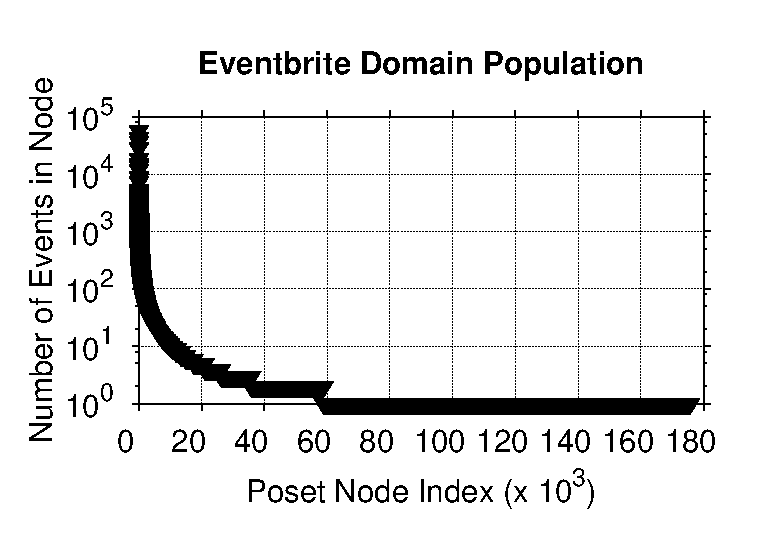
\includegraphics[clip,scale=0.5]{figs/eventbritepop.eps}
	\vspace{-15pt}
	\caption{The attributes describing the events domain and the hierarchical structure of each attribute.}
	\label{fig:eventbritepop}
	\vspace{-20pt}
	\end{center}
\end{figure}
As mentioned before, a critical challenge in such large domains is deciding on the queries to ask. However, the hierarchical structure of the data domain presents us with an opportunity. One approach would be to perform a top-down traversal of the poset and issue queries at the different nodes. Nevertheless, this gives rise to a series of challenges: (i) how can one decide on the number of queries to be asked at each node, (ii) when should one progress to deeper levels of the poset and (iii) which subareas should be explored. We elaborate on these in \Cref{sec:prelims}. Next, we focus on the second challenge, i.e., the interdependencies across poset nodes. 
\begin{example}
We consider again the Eventbrite dataset and plot the pairwise overlaps of the ten most populous nodes in the domain. \Cref{fig:eventbriteover} shows the Jaccard index for the corresponding node pairs. As shown the event populations corresponding to these nodes overlap significantly. It is easy to see that when issuing queries at a certain domain node, we not only obtain events corresponding to this node but to other nodes in the domain as well.
\end{example}
A critical issue that stems from the overlaps across nodes is being able to decide how many answers to expect when issuing an additional query at a node whose underlying population overlaps with nodes associated with previous queries. In \Cref{sec:prelims}, we elaborate more on the dependencies across nodes of the poset.

\begin{figure}
	\begin{center}
	\vspace{-10pt}
	\includegraphics[clip,scale=0.5]{figs/overlaps.eps}
	\vspace{-10pt}
	\caption{Pairwise overlaps for the 10 most populous nodes.}
	\label{fig:eventbriteover}
	\vspace{-20pt}
	\end{center}
\end{figure}

\subsection{Contributions}
\label{sec:contributions}
Motivated by the examples above, we study the problem of entity extraction over {\em structured domains}. More precisely, we focus on domains described by a collection of attributes, each following a known {\em hierarchical structure}, i.e., we assume that for each attribute the corresponding hierarchy is known. Such hierarchies are usually dictated by the design of applications. Moreover, as controlling the overall extraction cost in large-scale applications is crucial we focus on {\em budgeted crowd entity extraction}. 

We propose a novel algorithmic framework that exploits the structure of the domain to maximize the number of extracted entities under given budget constraints. In particular, we view the problem of entity extraction as a {\em multi-round adaptive optimization problem}. At  each round we exploit the information on extracted entities obtained by previous queries to adaptively select the crowd query that will maximize the {\em gain} and cost trade-off at each round. The gain of a query is defined as the {\em number of new unique entities extracted by it}. We extend on previous query interfaces that considered only questions of the type ``Give me $k$ more entities from a domain" and examine {\em generalized queries} that can also include an {\em exclude list}. In general such queries are of the type ``Give me $k$ more entities that from a domain that are not in $\{A, B, ...\}$". Extending techniques from the species estimation and building upon the multi-armed bandits literature, we introduce a new methodology for estimating the gain for such generalized queries and show how the hierarchical structure of the domain can be exploited to increase the number of extracted entities. Our main contributions are as follows:

\squishlist
\item We study the challenge of information flow across entity extraction queries for overlapping parts of the data domain.
\item We formalize the notion of an exclude list for crowdsourced entity extraction queries and show how previously proposed gain estimators can be extended to handle such queries.
\item We develop a new technique to estimate the gain of generalized entity extraction queries under the presence of dependent information. We empirically demonstrate the effectiveness of the proposed technique when extracting entities from sparse domains where little to no information is available for many nodes.
\item We introduce an adaptive optimization algorithm that takes as input the gain estimates for different types of queries and identifies querying policies that maximize the total number of retrieved entities under given budget constraints. 
\item Finally, we show that our techniques can effectively solve the problem of budgeted crowd entity extraction for large data domains on both real-world and synthetic data.
\squishend


%!TEX root = ../crowd_hierarchies_v.1.3.tex

\section{Preliminaries}
\label{sec:prelims}
In this section we first describe our structured data domain, then describe entities and entity extraction queries or interfaces, along with the response and cost model for these queries. The we focus on crowdsourced entity extraction using these interfaces and consider the problem of maximizing the number of extracted entities. In particular, we define the problem of {\em crowd entity extraction} over {\em structured domains} under budget constraints. Then, we formally introduce the challenge of dependencies across queries when extracting entities from structured domains, and finally, we present an overview of our proposed algorithmic framework. \agp{revisit}


\subsection{Structured Data Domain}
\label{sec:data-domain}

Let $\domain$ be a data domain described by a set of discrete attributes $\attributes = \{A_1, A_2, \dots, A_d\}$. Let $dom(A_i)$ denote the domain of each attribute $A_i  \in \attributes$. We focus on domains where each attribute $A_i$ is hierarchically organized. For example, consider the Eventbrite domain introduced in \Cref{sec:challenges}. The data domain $\domain$ corresponds to all events and the attributes describing the entities in $\domain$ are $\attributes = \{$``Event Type", ``Location", ``Date"$\}$. \Cref{fig:eventsdomain} shows the hierarchical organization of each attribute.

\begin{figure}[h]
	\begin{center}
	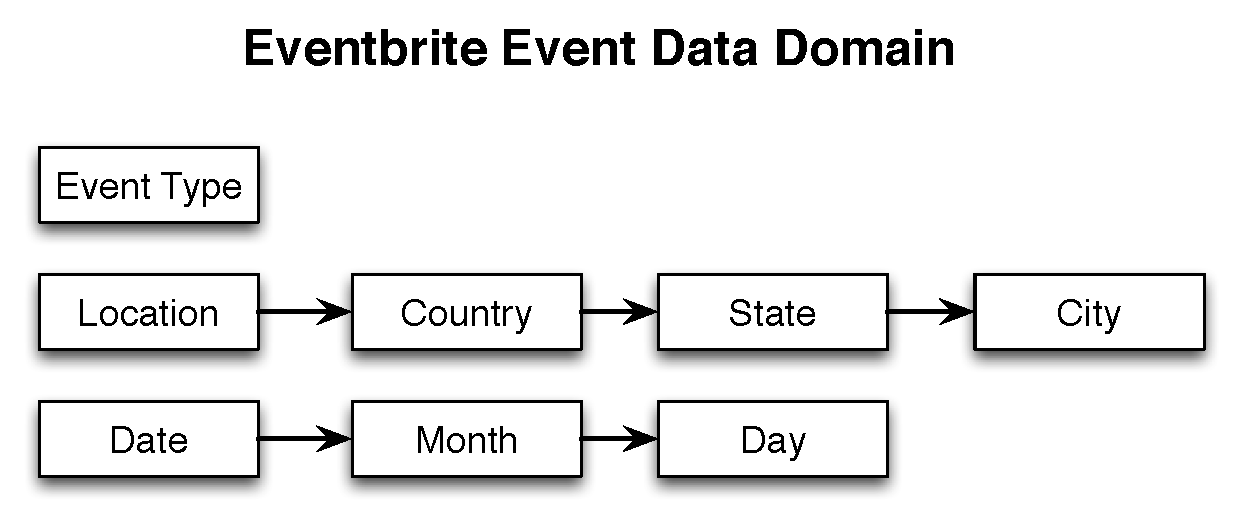
\includegraphics[clip,scale=0.4]{figs/eventsDomain.eps}
	\caption{The attributes describing the Eventbrite domain and the hierarchical structure of each attribute.}
	\label{fig:eventsdomain}
	\end{center}
	\vspace{-10pt}
\end{figure}

The domain $\domain$ can be viewed as a {\em poset}, i.e., a partially ordered set, corresponding to the cross-product of all available hierarchies\footnote{Note that $\domain$ is not a lattice since there is no unique infimum.}. Part of the poset corresponding to the previous example is shown in \Cref{fig:eventslattice}. We denote this cross-product as $\hierarchy$. As can be seen in \Cref{fig:eventslattice}, there are nodes, such as $\{\}$, where no attributes are specified, and nodes, such as $\{X1\}$ and $\{C1\}$ where just one of the attribute values is specified, as well as nodes, such as $\{X2, ST2\}$, where multiple attribute values are specified.



% We define a {\em point} in $\domain$ as a possible combination of values of {\em all} attributes: in our setting, if values are specified for all. We will also refer to a collection of points for which only a subset of attributes shares the same value as a {\em slice} $\domain_P$ of $\domain$. For example, a slice of the event domain described above may correspond to concerts in Boston. The predicates describing this slice are EVENT TYPE = ``Concert", LOCATION = ``Boston, MA", DATE = ``*".  It is easy to see that each node in $\hierarchy$ represents a slice of the data domain $\domain$. 

\begin{figure}[h]
	\begin{center}
	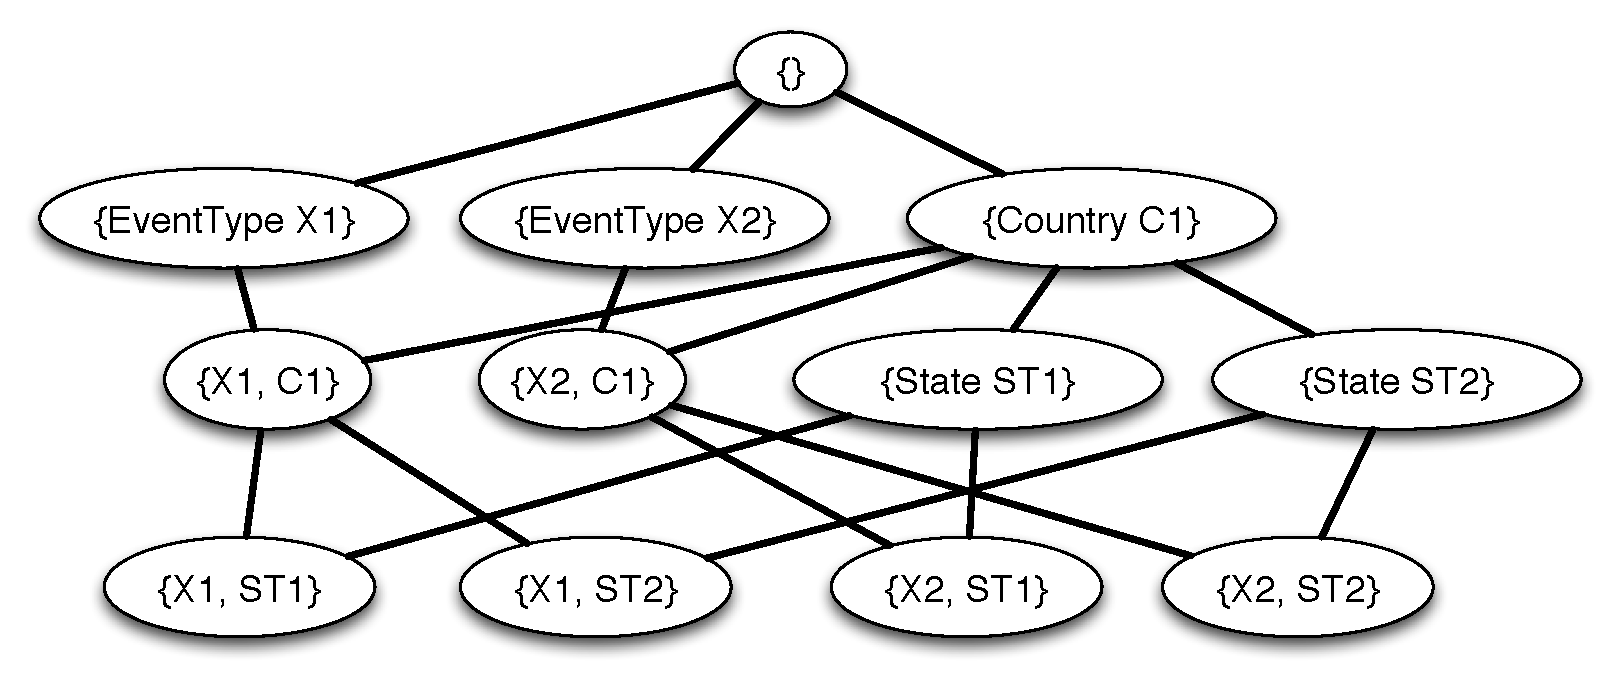
\includegraphics[clip,scale=0.32]{figs/eventsExLattice.eps}
	\caption{Part of the poset defining the entire event entity domain described by the attributes in \Cref{fig:eventsdomain}.}
	\label{fig:eventslattice}
	\end{center}
	\vspace{-10pt}
\end{figure}


\subsection{Entities and Entity Extraction Queries}
\label{sec:queries}

\stitle{Entities.} Our goal is to extract entities that belong to the domain $\domain$. We assume that each entity $e$ can be uniquely associated with one of the leaf nodes in the hierarchy $\hierarchy$; that is, there is a unique set of ``most-specific'' values of $A_1, \ldots, A_d$ for every entity. For example, in our Eventbrite dataset, each entity (here, a local event) takes place in a specific city, and on a specific day. Our techniques also work for the case when entities can be associated only with ``higher level'' nodes, but we focus on the former case for simplicity.

\stitle{Queries.} Next, we describe queries for extracting entities from the crowd; there are three different types of queries. The first type corresponds to {\em single entity queries} where workers are required to provide ``one more" entity that satisfies the collection of predicates over attributes in $\attributes$. Considering the Eventbrite example introduced in the previous section an example of a single entity query would be asking a worker to provide ``a concert in Manhattan, New York'". The second type of query corresponds to {\em queries of size k} where workers are asked to provide up to $k$ distinct entities. Finally, the last type corresponds to {\em exclude list queries}. Here,  workers are provided with $l$ entities that have already been extracted and are required to provide up to $k$ distinct entities under the constraint that none of them is included in this exclude list of size $l$. It is easy to see that the last type of query generalizes the previous two. Therefore, in the remainder of the paper, we will only consider queries of the third type. To describe a query, we will use the notation $q(k,l)$ denoting a query of size $k$ accompanied with an exclude list of length $l$. 

\stitle{Query Response.} Given a query $q(k, l)$, with an exclude list of entities $S, |S| = l$, a human worker gives us $k$ distinct entities that belong to the domain $\domain$, and are not present in $S$. Furthermore, the human worker provides us the information for the attributes that are not specified in $q$ for each of the $k$ entities. For example, if our query is ``a concert in Manhattan, New York'', with $k = 1, l = 0$, the human worker gives us one concert in Manhattan, New York, but also gives us the day on which the concert will take place (here, the missing, unspecified attribute). If the query is ``a concert in the US'', with $k = 1, l = 0$, the human worker gives us one concert in the US, but also gives the day on which the concert will take place, as well as the specific city. 

While the reader may wonder if getting additional attributes for entities is necessary, note that this information allows us to reason about which all nodes in $\hierarchy$ the entity belongs to; without this, it is impossible to effectively traverse the poset. Furthermore, we find that in most practical applications, it is useful to get the values of the missing attributes in order to organize and categorize the extracted entities better. 

Notice also that we assume that human workers specify or extract an entity correctly (e.g., no abbreviations, typos, and so on), once again for simplicity. It is straightforward to use an entity resolution algorithm to group identical entities together. Furthermore, since we are getting all attributes for each entity, we can use these attributes to further ascertain similarity of entities. In our experiments on real datasets, we found that there were no cases where humans introduced errors when extracting entities. 

\stitle{Query Cost.} In a typical crowdsourcing marketplace, tasks have different costs depending on their difficulty. Thus, crowdsourced queries of different difficulties should also exhibit different costs. Let $c(\dot)$ be a cost function for any query $q(k,l)$. This cost function should obey the following properties: (a) given an exclude list of fixed length $l$ then $c(q(k^{\prime},l)) \geq c(q(k,l)),  \forall k^{\prime} \geq k$, and (b) given a fixed query size $k$ then $c(q(k,l^{\prime})) \geq c(q(k,l)), \forall l^{\prime} \geq l$. These are fixed upfront by the interface designer based on the amount of work involved.

\subsection{Crowd Entity Extraction}
\label{sec:extraction}


The basic version of {\em crowd entity extraction}~\cite{trushkowsky:2013} seeks to extract entities that belong in a {\em single} slice $\domain_P$ of $\domain$, specified by a set of predicates $P$ over a subset of attributes in $\attributes$. However, when considering large entity domains, such as the event domain, one may need to issue a series of entity extraction queries over multiple slices of $\domain$ - that may overlap with each other- so that the entire domain is covered. Issuing queries for different slices of the domain ensures that the coverage across the domain will be maximized. 

Let $\mathcal{P}(\domain)$ denote the set of all possible slices that their union covers the domain $\domain$. Moreover, let $\pi$ denote a {\em querying policy}, that is, a chain of crowd queries corresponding to different slices in $\mathcal{P}(\domain)$. Each query asks workers to provide entities corresponding to a slice $\domain_P$. Notice, that multiple queries can be issued against the same slice. Let $C(\pi)$ denote the overall cost, both in terms of monetary cost and latency, of a querying policy $\pi$. We define the gain of a querying policy $\pi$ as the total number of unique entities, denoted by $\uentities(\pi)$ extracted when following policy $\pi$. 

The above naturally gives raise to a tradeoff between the total number of extracted entities and the total cost. To optimize this tradeoff, previous work has proposed either a {\em pay-as-you-go} scheme~\cite{trushkowsky:2013} or a fixed answer size scheme~\cite{park:2014}. In the first case, one repeatedly issues queries to the crowd until the {\em marginal gain}, i.e., the difference between the new extracted entities and the querying cost, drops below a desired threshold. However, the proposed scheme does not enforce any budget constraints explicitly and focuses on a single query in isolation. Thus, it does not optimize the gain-cost tradeoff over an entire querying policy. In the second case, one repeatedly issues queries to the crowd until a desired number of entities is retrieved. The latter is specified by the user. Notice, that this assumes knowledge of the number of entities to be extracted, nevertheless, this information may not be available in many real-world scenarios. 

Here, we require that the user will {\em only} provide a monetary budget $\tau_c$ imposing a constraint on the total cost of a selected querying policy, and optimize over all possible querying policies across different slices of the data domain. Our goal is to identify the policy that maximizes the number of retrieved entities under the given budget constraint. More formally, we define the problem of budgeted crowd entity extraction as follows:

\begin{definition}[Budgeted Crowd Entity Extraction]
Let $\domain$ be a given entity domain and $\tau_c$ a monetary budget on the total cost of issued queries. The Budgeted Crowd Entity Extraction problem seeks to find 
a querying policy $\pi^*_S$ over a subset of slices $S \subseteq \mathcal{P}(\domain)$ that maximizes the number of unique entities extracted $\uentities(\pi^*_S)$ under the constraint $C(\pi^*_S) \leq \tau_c$.
\end{definition}

If $\domain$ is fully specified by a hierarchy $\hierarchy$ then $\mathcal{P}(\domain) = \hierarchy$. Thus, determining the optimal querying policy requires detecting the optimal subset of nodes in $\hierarchy$ to be queried so that the goal number of extracted entities is maximized under the given budget constraint. Notice that due to the different query configurations the optimal querying policy for the problem of budgeted crowd entity extraction should also identify the optimal configuration $(k,l)$ for each query in $\pi^*_S$.

The cost of a querying policy $\pi$ is defined as the total cost of all queries issued by following $\pi$. We have that $C(\pi) = \sum_{q \in \pi} c(q)$ where the cost of each query $q$ is defined according to a cost model specified by the user. Computing the total cost of a policy $\pi$ is easy. However, the gain $\uentities(\pi)$ of a policy $\pi$ is unknown as we do not know in advance the entities corresponding to each node in $\hierarchy$, and hence, needs to be estimated, as we discuss next. 

\subsection{Queries in Structured Domains}
\label{sec:sampling}
The entities in the domain are unknown. Moreover, we assume that the underlying entities exhibit different {\em popularity levels} with respect to crowd workers. These popularity levels can be formally defined using the notion of a probability distribution. In particular, the probability that an entity will appear in a query depends on its {\em popularity} in the overall entity population. The popularity of an entity is defined as the probability that this entity will appear in a query $q(1,0)$, i.e., a query asking for one entity from the population and using an exclude list of size zero. Since workers are asked to provide a limited number of entities as response to a query, each entity extraction query can be viewed as taking a random sample from an unknown population of entities. In the remainder of the paper, we will refer to the distribution characterizing the popularities of entities corresponding to a population as the {\em popularity distribution} of the population. 

Estimating the gain of a query $q(k,l)$ at a node $v \in \hierarchy$ is equivalent to estimating the number of new entities extracted by taking additional samples from the population of $v$ given all the retrieved entities by past samples associated with node $v$~\cite{trushkowsky:2013}. 

When extracting entities from a structured domain, the retrieved entities for a node $v$ can correspond to two different kinds of samples: (i) those that were extracted by considering the {\bf entire population} corresponding to node $v$ (ii) and those that we obtained by sampling {\bf only a part of the population} corresponding to $v$. Samples for a node $v$ can be obtained either by querying node $v$ or by indirect information flowing to $v$ by queries at other nodes in $\hierarchy$. We refer to the latter case as {\em dependencies across queries}. 
\begin{figure}[h]
	\begin{center}
	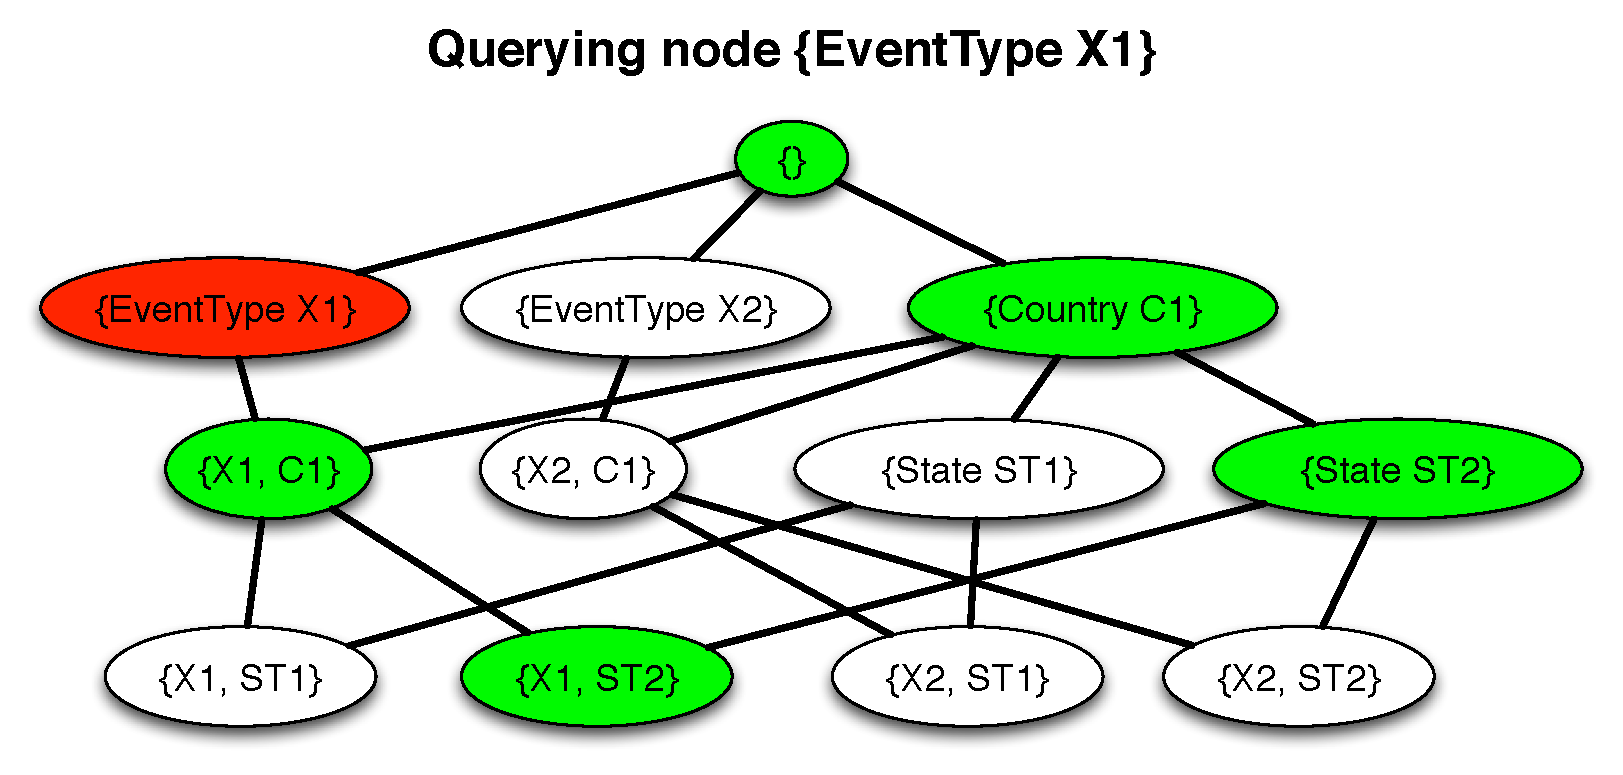
\includegraphics[clip,scale=0.32]{figs/exampleQuery.eps}
	\caption{An example query that extract an entity sample from the red node. The nodes marked with green correspond to the nodes for which indirect entity samples are retrieved.}
	\label{fig:query}
	\end{center}
	\vspace{-10pt}
\end{figure}

We use an example considering the poset in \Cref{fig:eventslattice}, to illustrate these two cases. The example is shown in \Cref{fig:query}. Assume a query $q(k,0)$ issued against node \{EventType X1\}. Assume that the query result contains entities that correspond only to node \{X1,ST2\}. The green nodes in \Cref{fig:query} are nodes for which samples are obtained indirectly without querying them. Notice, that all these nodes, are ancestors of \{X1,ST2\}. Analyzing the samples for the different nodes we have:
\squishlist
\item The samples corresponding to nodes \{X1, C1\} and \{X1,ST2\} where obtained by considering their {\em entire population}. The reason is that node \{EventType X1\} is an ancestor of both and the entity population corresponding to it fully contains the populations of both \{X1,C1\} and \{X1,ST1\}. 
\item The samples corresponding to nodes \{ \}, \{Country C1\} and \{State ST2\} where obtained by considering only part of their population. The reason is that the population of node \{EventType X1\} does not fully contain the populations of these nodes. 
\squishend

Samples belonging to both types need to be considered when estimating the gain of a query at a node in $v \in \hierarchy$. To address this issue we merge the extracted entities for each node in $\hierarchy$ into a single sample and treat the unified sample as being extracted from the entire underlying population of the node. As we discuss later in \Cref{sec:solving} we develop querying strategies that traverse the poset $\hierarchy$ in a top-down approach, hence, the number of samples belonging in the first category, i.e., samples retrieved considering the entire population of a node, dominates the number of samples retrieved by considering only part of a node's population. Moreover, it has been shown by Hortal et al.~\cite{hortal2006evaluating} that several of the techniques that can be used to estimate the gain of a query(see \Cref{sec:gainestimators}) present insensitivity to differences in the way the samples are aggregated.

\subsection{Framework Overview}
\label{sec:framework}
We present an overview of our proposed framework for solving the problem of budgeted crowd entity extraction over structured domains. We view the optimization problem described in \Cref{sec:extraction} as a multi-round adaptive optimization problem where at each round we solve the following subproblems: 
\squishlist 
\item \textbf{Estimating the Gain for a Query.} For each node in $v \in \hierarchy$, consider the retrieved entities associated with $v$ and estimate the number of new unique entities that will be retrieved if a new query $q(k,l)$ is issued at $v$. This needs to be repeat for all possible configurations of $k$ and $l$.
\item \textbf{Detecting the Optimal Querying Policy.} Using the gain estimates from the previous problem as input, identify the next (query, node) combination so that the total gain across all rounds is maximized with respect to the given budget constraint. 
\squishend
Our proposed framework iteratively solves the aforementioned problems until the entire budget is used. \Cref{fig:framework} shows a high-level diagram of our proposed framework. Throughout our framework, we assume that after issuing a query against the crowd, the retrieved answers can be associated with all relevant nodes across all attribute hierarchies, i.e., a worker will provide all the attribute values describing a reported entity. Dealing with incomplete information about entities is not the main focus of this paper and is part of the future work preposed in \Cref{sec:conclusions}.

\begin{figure}
	\begin{center}
	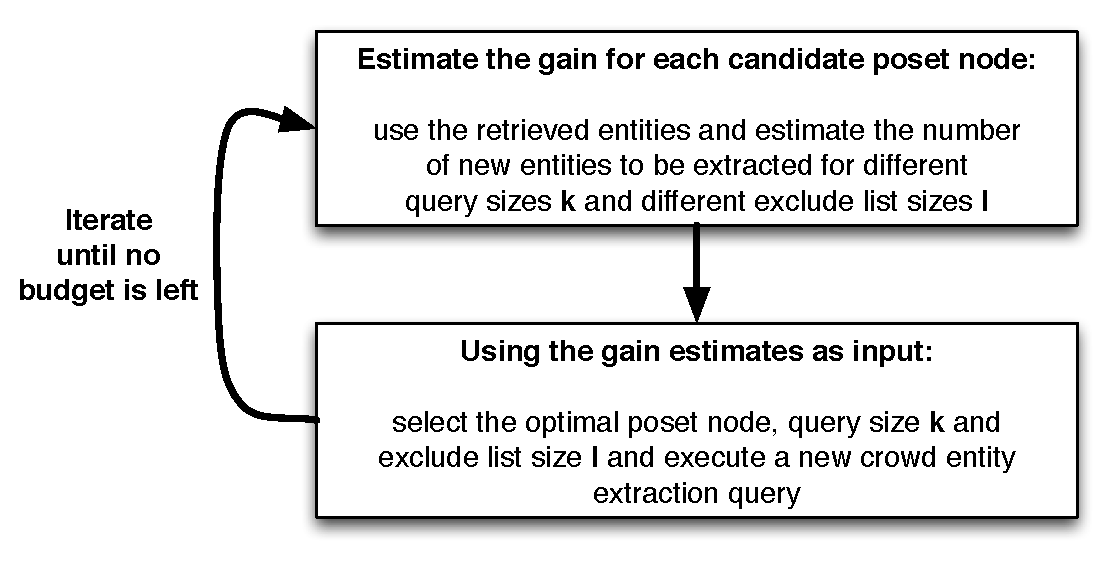
\includegraphics[clip,scale=0.45]{figs/framework.eps}
	\caption{Solution overview for budgeted entity extraction.}
	\label{fig:framework}
	\end{center}
	\vspace{-10pt}
\end{figure}

%!TEX root = ../crowd_hierarchies_v.1.3.tex


\section{Estimating the Gain of Queries}
\label{sec:gainestimators}
We now present a novel estimation technique for the return of a generalized query $q(k,l)$ at a node $v \in \hierarchy$. Previous work~\cite{trushkowsky:2013} has drawn connections between this problem and species estimation literature~\cite{chao:1992}. However,  these techniques really on the presence of a relatively large sample and are agnostic to the presence of an exclude-list-based query interface. In particular, there is no mechanism for estimating the number of new tuples extracted by a query when restricting the worker answer to not contain any entities from a certain collection of entities as enforced by an exclude list. We first review the existing methodology for estimating the gain of a query, then we discuss how these estimators can be extended to consider an exclude list, and finally, we present a new methodology for estimating the gain of generalized queries $q(k,l)$ directly under the presence of little information. 

\subsection{Previous Estimators} 
Consider a specific node $v \in \hierarchy$. Prior work only considers samples retrieved from the entire population associated with $v$ and does not consider an exclude list. Let $Q$ be the set of all existing samples retrieved by issuing queries against $v$ without an exclude list. These samples can be combined into a single sample of size $n = \sum_{q \in Q} {\sf size}(q)$. Let $f_i$ denote the number of entities that appear $i$ times in this unified sample, and let $f_0$ denote the number of unseen entities from the population under consideration. Finally, let $C$ be the population coverage of the unified sample --- that is, this is the fraction of the population covered by the sample.

A new query $q(k,0)$ at node $v$ can be viewed as increasing the size of the unified sample by $k$. Prior work used techniques from species estimation to estimate the expected number of new entities returned in $q(k,0)$. Shen et al.~\cite{shen:2003}, derive an estimator for the number of new species $\hat{N}_{Shen}$ that would be found in an increased sample of size $k$. The approach assumes that the unobserved entities have equal relative popularity. An estimate of the unique elements found in an increased sample of size $k$ is given by:
\begin{equation}
\label{eq:shen}
\hat{N}_{Shen} = f_0\left( 1 - \left(1 - \frac{1 - C}{f_0}\right)^k\right)
\end{equation}
At a high-level, the second term of Shen's formula corresponds to the probability that at least one unseen entity will be present in a query asking for $k$ more entities. Thus, multiplying this quantity with the number of unseen entities $f_0$ corresponds to the expected number of unseen entities that will be present in the result of a new query $q(k,0)$.

Notice, that the quantities $f_0$ and $C$ are unknown and thus need to be estimated considering the entities in the running unified sample. The coverage can be estimated by considering the Good-Turing estimator $\hat{C} = 1 - \frac{f_1}{n}$ for the existing retrieved sample. On the other hand, multiple estimators have been proposed for estimating the number of unseen entities $f_0$. Trushkowsky et al.~\cite{trushkowsky:2013} proposed a variation of an estimator introduced by Chao et al.~\cite{chao:1992} to estimate $f_0$. Nevertheless, the authors argue that the original estimator proposed by Chao performs similarly with their approach when estimating the gain of an additional query $q(k,0)$.

The estimator by Chao~\cite{chao:1992} upon which the authors build has been shown to result in considerable bias in cases where the number of observed entities from a population represents only a {\em small fraction} of the entire population~\cite{hwang:2010}. Notice, that this assumption holds for crowdsourced entity extraction in a large domain, i.e., we are observing only a small portion of the entire population.  To address this problem, Hwang and Shen~\cite{hwang:2010} proposed a regression based technique to estimate $f_0$. This estimator is shown to result in significantly smaller bias and empirically outperforms previously proposed estimators, including the one proposed by Chao, when the ratio of retrieved entities to the entire entity population is small. It also performs comparably to previous estimators when the ratio is larger. Notice that the output of this estimator can also be used as a plug-in quantity in \Cref{eq:shen}. 
%Thus, in this paper, we use the regression based estimator proposed by Hwang and Shen~\cite{hwang:2010}; in \Cref{sec:exps} we empirically show that it is better than the one proposed by Chao~\cite{chao:1992}.

However, both the aforementioned estimators are agnostic to an exclude list. Next, we discuss how one can estimate the return of a query $q(k,l)$ in the presence of an exclude list of size $l$.
\subsection{Queries With an Exclude List}
\label{sec:excludelist}
Consider an exclude list of size $l$. As discussed before an exclude list is a set of entities that correspond to invalid worker answers. Considering an exclude list for a query at a node $v \in \hierarchy$ corresponds to limiting our sampling to a restricted subset of the entity population corresponding to node $v$. In fact, we want to estimate the expected return of a query of size $k$ conditioning on the fact that the entities in the exclude list will not be retrieved by any new sample. The latter corresponds to removing these entities from the population under consideration. Thus, the estimates $\hat{f}_0$ and $\hat{C}$ should be updated before applying \Cref{eq:shen} to compute the expected return of a query of size $k$. This can be done by removing the entities included in the exclude list from the running sample for node $v$, recomputing the entity counts $f_i$ and following the techniques presented above for computing the updated estimates for $\hat{f}_0$ and $\hat{C}$. This approach requires that the exclude list is known in advance. To construct an exclude list one can follow a randomized approach, where $l$ of the retrieved entities are included in the list uniformly at random. The generated list can be used to update the frequency counts $f_i$ and estimate the gain of the query. Bootstrapping can also be used to obtain improved estimates.

\subsection{Regression Based Gain Estimation}
\label{sec:newestim}
Building upon the approach of Hwang and Shen~\cite{hwang:2010}, we introduce a new technique for estimating the gain of a generalized query $q(k,l)$ directly without using the estimator shown in \Cref{eq:shen}. Since we want to estimate the gain even for nodes with a small number of retrieved entities we propose a regression based technique that is able to capture the structural properties of the expected gain function as discussed below. 

To derive the new estimator we make used of the generalized jackknife procedure for species richness estimation~\cite{heltshe1983estimating}. Given two (biased) estimators of $S$, say $\hat{S}_1$ and $\hat{S}_2$, let $R$ be the ratio of their biases:
\begin{equation}
R = \frac{E(\hat{S}_1) - S}{E(\hat{S}_2) - S}
\end{equation}
By the generalized jackknife procedure, we can completely eliminate the bias resulting from either $\hat{S}_1$ or $\hat{S}_2$ via
\begin{equation}
S = G(\hat{S}_1, \hat{S}_2) = \frac{\hat{S}_1 - R\hat{S}_2}{1 - R}
\label{eq:jknife}
\end{equation}
provided the ratio of biases $R$ is known. However, $R$ is unknown and needs to be estimated. 

Let $D_n$ denote the number of unique entities in a unified sample of size $n$. We consider the following two biased estimators of $S$: $\hat{S_1} = D_n$ and $\hat{S}_2 = \sum_{j=1}^n D_{n-1}(j)/n = D_n - f_1/n$ where $D_{n-1}(j)$ is the number of species discovered with the $j$th observation removed from the original sample. Replacing these estimators in \Cref{eq:jknife} gives us:
\begin{equation}
S = D_n +\frac{R}{1-R}\frac{f_1}{n}
\end{equation}
Similarly, for a sample of increased size $n+m$ we have:
\begin{equation}
S = D_{n+m} +\frac{R^{\prime}}{1-R^{\prime}}\frac{f^{\prime}_1}{n+m}
\end{equation}
where $R^{\prime}$ is the ratio of the biases and $f^{\prime}_1$ the number of singleton entities for the increased sample. Let $K = \frac{R}{1-R}$ and $K^{\prime} = \frac{R^{\prime}}{1-R^{\prime}}$. Taking the difference of the previous two equations we have:
\begin{equation}
D_{n+m} - D_{n} = K\frac{f_1}{n} - K^{\prime}\frac{f^{\prime}_1}{n+m}
\end{equation}
Therefore, we have:
\begin{equation}
\label{eq:new}
new = K\frac{f_1}{n} - K^{\prime}\frac{f^{\prime}_1}{n+m}
\end{equation}
We need to estimate $K$, $K^{\prime}$ and $f^{\prime}_1$. We start with $f^{\prime}_1$, which denotes the number of singleton entities in the increased sample of size $n+m$. Notice, that $f^{\prime}_1$ is not known since we have not obtained the increased sample yet, so we need to express it in terms of $f_1$, i.e., the number of singletons, in the running sample of size $n$. We have:
\begin{equation}
f^{\prime}_1 = new + f_1 - f_1^c
\end{equation}
where $f_1^c$ denotes the number of old singleton entities from the sample of size $n$ that appeared in the additional query of size $m$. Let $E_1$ denote the set of singleton entities in the old sample of size $n$. We approximate $f_1^c$ by its expected value:
\begin{equation}
\hat{f}_1^c = \sum_{e \in E_1} \Pr[\mbox{e appears in query of size $m$}]
\end{equation}
We compute the probability of an old singleton entity appearing in an additional query as follows. Let $p_e$ denote the popularity of entity $e$. As described before, an additional query of size $m$ corresponds to taking a sample of size $m$ from the underlying entity population without replacement. However, $m$ is significantly smaller compared to the size of the underlying population, thus, we can consider a that taking a sample of size $m$ corresponds to taking a sample {\em with replacement}. Following this we have that:
\begin{equation}
\Pr[\mbox{e appears in query of size $m$}] = 1 - (1-p_e)^m
\end{equation}
Following a standard approach in the species estimation literature we assume that the popularity of retrieving a singleton entity again is the same for all singleton entities. This popularity can be computed using the corresponding Good-Turing estimator considering the running sample. We have:
\begin{equation}
\forall e \in E_1, p_e = p_1 = \hat{\theta}(1) = \frac{1}{n}2\frac{N_2}{N_1}
\end{equation}
where $N_2$ is the number of entities that appear twice in the sample and $N_1$ is the number of singletons. 
Eventually we have that:
\begin{equation}
\hat{f}_1^c = f_1(1 - (1-p_1)^m)
\end{equation}
and
\begin{equation}
f^{\prime}_1 = new + f_1(1-p_1)^m
\end{equation}
Replacing the last equation in \Cref{eq:new} we have:
\begin{align}
&new = K\frac{f_1}{n} - K^{\prime}\frac{new + f_1(1-p_1)^m}{n+m} \nonumber \\
%&new = K\frac{f_1}{n} - K^{\prime}\frac{new}{n+m} - K^{\prime}\frac{f_1(1- P)}{n+m} \nonumber \\
%&new(1 + \frac{K^{\prime}}{n+m}) = K\frac{f_1}{n} - K^{\prime}\frac{f_1(1- P)}{n+m} \nonumber \\
&new = \frac{1}{(1 + \frac{K^{\prime}}{n+m})}(K\frac{f_1}{n} - K^{\prime}\frac{f_1(1-p_1)^m}{n+m}) \nonumber
\end{align}
Next, we discuss how one can estimate $K$ and $K^{\prime}$. To estimate $K$ we follow the regression approach introduced by Hwang and Shen~\cite{hwang:2010}. From the Cauchy-Schwarz inequality we have that:
\begin{equation}
K = \frac{\sum_{i=1}^S (1-p_i)^n}{\sum_{i=1}^S p_i(1-p_i)^{n-1}} \geq \frac{(n-1)f_1}{2f_2}
\end{equation}
This can be generalized to:
\begin{equation}
K=\frac{nf_0}{f_1} \geq \frac{(n-1)f_1}{2f_2} \geq \frac{(n-2)f_2}{3f_3} \geq \dots
\end{equation}
Let $g(i) = \frac{(n-i)f_i}{(i+1)f_{i+1}}$. From the above we have that the function $g(x)$ is a smooth monotone function for all $x \geq 0$. Moreover, let $y_i$ denote a realization of $g(i)$ mixed with a random error. Hwang and Shen how one can use an exponential regression model to estimate $K$. The proposed model corresponds to:
\begin{equation}
y_i = \beta_0\exp(\beta_1i^{\beta_2}) + \epsilon_i
\end{equation}
where $i = 1, \dots, n-1$, $\beta_0 > 0$, $\beta_1 < 0$, $\beta_2 >0$ and $\epsilon_i$ denotes random errors. It follows that $K = \beta_0$. 

Finally, we show how one can estimate the value of $K^{\prime}$ for an increased sample of size $n+m$. First, we show that $K$ increases monotonically as the size of the running sample increases. Let $K(n) = \frac{\sum_{i=1}^S (1-p_i)^n}{\sum_{i=1}^S p_i(1-p_i)^{n-1}}$ be a function returning the value of $K$ for a sample of size $n$. We have the following lemma. 

\begin{lemma}
We have $K(n+m) \geq K(n), \forall n,m > 0$.
\end{lemma}
\begin{proof}
In the remainder of the proof we will denote $K(n+m)$ as $K^{\prime}$. By definition we have that $K = \frac{\sum_{i=1}^S (1-p_i)^n}{\sum_{i=1}^S p_i(1-p_i)^{n-1}}$ and $K^{\prime} = \frac{\sum_{i=1}^S (1-p_i)^{n+m}}{\sum_{i=1}^S p_i(1-p_i)^{n+m-1}}$. We want to show that:

{\small
\begin{align}
&\frac{\sum_{i=1}^S (1-p_i)^{n+m}}{\sum_{i=1}^S p_i(1-p_i)^{n+m-1}} \geq \frac{\sum_{i=1}^S (1-p_i)^n}{\sum_{i=1}^S p_i(1-p_i)^{n-1}} \nonumber \\
&\sum_{i=1}^S (1-p_i)^{n+m}\sum_{j=1}^S p_j(1-p_j)^{n-1} \geq \sum_{i=1}^S p_i(1-p_i)^{n+m-1}\sum_{j=1}^S (1-p_j)^n\nonumber \\
&\sum_{i,j:i\prec j}[(1-p_i)^{n+m}p_j(1-p_j)^{n-1} - p_i(1-p_i)^{n+m-1}(1-p_j)^n + \nonumber \\
& + (1-p_j)^{n+m}p_i(1-p_i)^{n-1} - p_j(1-p_j)^{n+m-1}(1-p_i)^n] \geq 0 \nonumber \\
%&\sum_{i,j:i\prec j}[(1-p_i)^{n}(1-p_j)^{n-1}p_j((1-p_i)^{m} - (1-p_j)^{m})  + \nonumber \\
%& - (1-p_j)^{n}p_i(1-p_i)^{n-1}((1-p_i)^{m} - (1-p_j)^{m}) \geq 0 \nonumber \\
&\sum_{i,j:i\prec j}[(1-p_i)^{n-1}(1-p_j)^{n-1}(p_j-p_i)((1-p_i)^{m} - (1-p_j)^{m}) \geq 0
\end{align}}

But the last inequality always holds since each term of the summation is positive. In particular, if $p_j \geq p_i$ then
also $1-p_i \geq 1-p_j$ and if $p_j \leq p_i$ then $1-p_i \leq 1-p_j$.
\end{proof}

We have that $K(n)$ is an increasing function of the sample size. Moreover, $K(n)$ has a decreasing slope. We model $K$ as a generalized logistic function of the form $f(x) = \frac{A}{1+exp(-G(x-D))}$. As we observe samples of different sizes for different queries we estimate $K$ as described above and therefore we observe different realizations of $f(\cdot)$. Thus, we can learn the parameters of $f$ and use it to estimate $K^{\prime}$. In the presence of an exclude list of size $l$ we follow the approach described in \Cref{sec:excludelist} to update the quantities $f_i$ used in the analysis above. 

\subsection{Negative Answers and Gain Estimation}
\label{sec:neg}
Next, we study the effect of {\em negative answers} on estimating the gain of future queries. It is possible to issue a query at a specific node $v \in \hierarchy$ and receive no entities, i.e., we receive a negative answer. This is an indication that the underlying entity population of $v$ is empty. In such a scenario, we assign the expected gain of future queries at $v$ and all its descendants to zero. 

Another type of negative answer corresponds to the scenario where we issue a query at an ancestor node $u$ of $v$ and receive no entities associated with $v$ but received some entities for $u$. Notice, that in this case, we do not have enough information to update our estimates for node $u$. The reason is that due to the restricted query size entities from other descendants of $u$ may be more popular with respect to the popularity distribution of $u$.
%\agp{this subsection is weird. can we combine with 3.2?}
%!TEX root = ../crowd_hierarchies_v.1.3.tex


\section{Discovering Querying Policies}
\label{sec:solving}
In this section, we focus on the second component of our proposed algorithmic framework. Specifically, we introduce a querying strategy based on a multi-round adaptive optimization algorithm to maximize the total gain across all rounds under the given budget constraints. The algorithmic framework we propose builds upon ideas from the multi-armed bandit literature~\cite{Auer:2003,EvenDar06actionelimination}. In particular, at each round, the proposed algorithm uses as input the estimated gain or return for queries $q(k,l)$ at the different nodes in $\hierarchy$. Before presenting our proposed algorithm we list several challenges associated with this adaptive optimization problem.

\squishlist
\item The first challenge is that the number of nodes in $\hierarchy$ is exponential with respect to the number of attributes $\attributes$ describing the domain of interest. Querying every possible node to estimate its expected return for different queries $q(k,l)$ is prohibitively expensive. That said, typical budgets do not allow algorithms to query all nodes in the hierarchy, so this intractability may not hurt us all that much. For example, we can keep estimates for each of the nodes for which at least one entity has been retrieved.
\item The second challenge is balancing the tradeoff between {\em exploitation} and {\em exploration}~\cite{Auer:2003}. The first refers to querying nodes for which sufficient entities have been retrieved and hence we have an accurate estimate for their expected return; the latter refers to exploring new nodes in $\hierarchy$ to avoid locally optimal policies.
\squishend

\subsection{Balancing Exploration and Exploitation}
While issuing different queries $q(k,l)$ at different nodes of $\hierarchy$ we obtain a collection of entities that can be assigned to different nodes in $\hierarchy$. For each node we can estimate the return of a new query $q(k,l)$ using the estimator presented in \Cref{sec:newestim}. However, this estimate is based on a rather small sample of the underlying population. Thus, exploiting this information at every round may lead to suboptimal decisions. This is the reason why one needs to balance the trade-off between exploiting nodes for which the estimated return is high and nodes that have not been queried many times. Formally, the latter corresponds to upper-bounding the expected return of each potential action with a confidence interval that depends on both the variance of the expected return and the number of times an action is evaluated.

Let $r(\alpha)$ denote the expected return of action $\alpha$ that is an estimate of the true return $r^*(\alpha)$. Moreover, let $\sigma(\alpha)$ be an error component on the return of action $\alpha$ chosen such that $r(\alpha) - \sigma(\alpha) \leq r^*(\alpha) \leq r(\alpha) + \sigma(\alpha)$ with high probability. The parameter $\sigma(\alpha)$ should take into account both the empirical variance of the expected return as well as our uncertainty if an action or similar actions (e.g., with different $k, l$ but at the same node) has been chosen few times. Let $n_{\alpha,t}$ be the number of times we have chosen action $\alpha$ by round $t$, and let $v_{\alpha,t}$ denote the maximum value between some constant $c$ (e.g., $c = 0.01$) and the empirical variance for action $\alpha$ at round $t$. The latter can be computed using bootstrapping over the retrieved sample and applying the estimators presented in \Cref{sec:newestim} over these bootstrapped samples. Several techniques have been proposed in the multi-armed bandits literature to compute the parameter $\sigma(\alpha)$~\cite{teytaud:inria-00173263}. Teytaud et al.~\cite{teytaud:inria-00173263} showed that techniques considering both the variance and the number of times an action has been chosen tend to outperform other proposed methods. Based on this observation, we choose to use the following formula for sigma:
\begin{equation}
\label{eq:upper}
\sigma(\alpha) = \sqrt{\frac{v_{\alpha,t}\cdot\log(t)}{n_{\alpha,t}}}
\end{equation}

\subsection{A Multi-Round Querying Policy Algorithm}
\label{sec:heuristic}
We now introduce our proposed multi-round algorithm for solving the budgeted entity enumeration problem. At a high-level, our algorithm proceeds as follows: Let $\mathcal{S}$ denote the set of all potential queries $q(k,l)$ that can be issued at the different nodes of $\hierarchy$ during a round $r$. Moreover, let $r(\alpha) + \sigma(\alpha)$ and $c(\alpha)$ be the upper-bounded return (i.e., gain) and cost for an action $\alpha \in \mathcal{S}$. At each round the algorithm identifies an action in $\mathcal{S}$ that maximizes the quantity $\frac{r(\alpha) + \sigma(\alpha)}{c(\alpha)}$ under the constraint that the cost of action $\alpha$ is less or equal to the remaining budget. Since we are operating under a specified budget one can view the problem in hand as a variation of the typical knapsack problem. If no such action exists then the algorithm terminates. Otherwise the algorithm issues the query corresponding to action $\alpha$, updates the set of unique entities obtained from the queries, the remaining budget and updates the set of potential queries $q(k,l)$ that can be executed in the next round.  An overview of the proposed algorithm is shown in Algorithm \ref{algo:overall}. 

As discussed before, the size of $\hierarchy$ is exponential to the values of attributes describing it, and thus, considering all the possible queries corresponding to the different nodes of the hierarchy can be prohibitively expensive. Next, we discuss how one can initialize and update the set of potential actions as the algorithm progresses considering the structure of the poset $\hierarchy$ and the retrieved entities from previous rounds. 

\begin{algorithm}[h]
\small\caption{Overall Algorithm}
\label{algo:overall}
\begin{algorithmic}[1]
\STATE {\bf Input:} $\hierarchy$: the hierarchy describing the entity domain; $r,\sigma$: value oracle access to gain upper bound; $c$: value oracle access to the query costs; $\beta_c$: query budget;
\STATE {\bf Output:} $\uentities$: a set of extracted distinct entities;
\STATE $\uentities \leftarrow \{\}$
\STATE $RB \leftarrow \beta_c$ /* Initialize remaining budget */
\STATE $\mathcal{S} \leftarrow$ {\sf UpdateActionSet($\hierarchy$)}
\WHILE {$RB > 0$ and $S \neq \{\}$}
	\STATE $\alpha \leftarrow \arg\max_{\alpha \in {\mathcal{S}}} \frac{r(\alpha)+\sigma(\alpha)}{c(\alpha)}$ such that $RB - c(\alpha) >0$
	\IF {$\alpha$ is NULL }
		\STATE break;
	\ENDIF
	\STATE $RB \leftarrow RB - c(\alpha)$ /* Update budget */
	\STATE Issue query corresponding to $\alpha$
	\STATE $E \leftarrow$ entities from query
	\STATE $\uentities \leftarrow \uentities \cup E$ /* Update unique entities */
	\STATE $\mathcal{S} \leftarrow$ {\sf UpdateActionSet($\hierarchy$)}
\ENDWHILE
\RETURN $\uentities$
\end{algorithmic}
\end{algorithm}

\subsection{Updating the Set of Actions}
Due to the exponential size of the poset $\hierarchy$, we need to limit the set of possible actions Algorithm~\ref{algo:overall} considers. To avoid keeping estimates for actions with bad returns we exploit the structure the given domain $\hierarchy$. We propose an algorithm that updates the set of actions by traversing the input poset in a top-down manner extending it by adding new actions that corresponds to queries for nodes that are {\em direct descendants} of already queried nodes.

The intuition behind this approach is the following. It is easy to see that due to the hierarchical structure of the poset nodes at higher levels of the poset correspond to larger populations of entities. Therefore, issuing queries at these nodes can potentially result to a larger number of extracted entities. Also, traversing the poset in a bottom-down fashion allows one to detect sparsely populated areas of the poset and hence avoid spending any of the available budget on issuing queries corresponding to them.

In more detail, our approach for updating the set of available actions (Algorithm~\ref{algo:updateactions}) proceeds as follows: If the set of available actions is empty start by considering all possible queries that can be issued at the root of $\hierarchy$ (Ln. 4-5). The set of possible queries corresponds to queries $q(k,l)$ for all combinations of the values of parameters $k$ and $l$. Recall that these are pre-specified by the designer of the querying interface. If the set of available actions is not empty, we consider the node associated with the action selected in the last round and populate the set of available actions with all the queries corresponding to its direct descendants (Ln. 7-9), i.e., by traversing the input poset in a bottom-down fashion. As mentioned above the number of nodes in $\hierarchy$ can be prohibitively large, therefore we also {\em remove} any {\em bad actions} from the running set of actions (Ln.  10-14). 
An action $\alpha$ is bad when $r(\alpha) + \sigma(\alpha) < \max_{\alpha^{\prime} \in \mathcal{S}} (r(\alpha^{\prime}) - \sigma(\alpha^{\prime}))$. Intuitively, this inequality states that we do not need to consider again an action as long as there exists another action such that the upper-bounded return of the former is lower than the lower bounded return of the latter. This is a standard technique adopted in multi-armed bandits to limit the number of actions considered by the algorithm~\cite{EvenDar06actionelimination}. 


\begin{algorithm}[h]
\small\caption{UpdateActionSet}
\label{algo:updateactions}
\begin{algorithmic}[1]
\STATE {\bf Input:} $\hierarchy$: the hierarchy describing the entity domain; $u$: a node in $\hierarchy$ associated with the last selected action; $\mathcal{S}_{old}$: the running set of actions; $V_k$: set of values for query parameter $k$; $V_l$: set of values for query parameter $l$;
\STATE {\bf Output:} $\mathcal{S}_{new}$: the updated set of actions;
\STATE \textbf{/* Extend Set of Actions*/}
\IF {$\mathcal{S}_{old}$ is empty}
	\RETURN $\{$Root of $\hierarchy \}$
\ENDIF 
\STATE $\mathcal{S}_{new} \leftarrow \mathcal{S}_{old}$
\FORALL{$d \in ${\sf ~Set of Direct Descendant Nodes of $u$ in $\hierarchy$}}
\STATE $A_d \leftarrow$ Set of queries at $u$ for all configurations in $V_k \times V_l$
\STATE $\mathcal{S}_{new} \leftarrow \mathcal{S}_{new} \cup A_d$
\ENDFOR
\STATE \textbf{/* Remove Bad Actions*/}
\STATE /* Find maximum lower bound on gain over all actions in $\mathcal{S}_{new}$*/
\STATE $thres \leftarrow \max_{\alpha^{\prime} \in \mathcal{S}_{new}} (r(\alpha^{\prime}) - \sigma(\alpha^{\prime}))$  
\STATE $\mathcal{B} \leftarrow$ All actions $a$ in $\mathcal{S}_{new}$ with $r(\alpha) + \sigma(\alpha) < thres$
\STATE $\mathcal{S}_{new} \leftarrow \mathcal{S}_{new} \setminus \mathcal{B}$
\RETURN $\mathcal{S}_{new}$
\end{algorithmic}
\end{algorithm}
\vspace{-20pt}
\section{Experimental Evaluation}
\label{sec:exps}
In this section we present an empirical evaluation of our proposed algorithmic framework. The main questions we seek to address are: (1) how the proposed querying policy algorithm compares against baselines for maximizing the number of extracted entities under a specific budget, (2) how the different gain estimators presented in \Cref{sec:gainestimators} compare with each other, and (3) how the proposed querying policy algorithm exploits the structure of the input domain to construct the set of available actions.

We empirically study these questions using both real and synthetic datasets. First, we discuss the experimental methodology, and then we describe the data and results that demonstrate the effectiveness of our framework on crowdsourced entity extraction. The evaluation is performed on an Inter(R) Cored(TM) i7 3.7 GHz/32GB machine. The proposed framework is implemented in Python 2.7. 

\vspace{5pt}\noindent\textbf{Gain Estimators:} We evaluate the following gain estimators:
\squishlist
\item Chao92Shen: This estimator combines the methodology proposed by Chao~\cite{chao:1992} for estimating the number of unseen species  with Shen's formula~\Cref{eq:shen}. This approach has been used by Trushkowsky et al.~\cite{trushkowsky:2013} in their evaluation.
\item HwangShen: This estimator combines the regression based approach proposed by Hwang and Shen~\cite{hwang:2010} for estimating the number of unseen species with Shen's formula. 
\item NewRegr: This estimator corresponds to the new regression based technique proposed in \Cref{sec:newestim}.
\squishend
All estimators were coupled with bootstrapping to estimate their variance. Computing the variance of each estimator is required to retrieve an upper bound on the return of a query as shown in \Cref{eq:upper}.

\vspace{5pt}\noindent\textbf{Entity Extraction Algorithms:} We evaluate the following algorithms for crowdsourced entity extraction:
\squishlist
\item Rand: This algorithm executes random queries over the input domain until all the available budget is used. It selects a random node from the input poset $\hierarchy$ and a random query configuration $q(k,l)$ from a list of pre-specified $k$, $l$ value combinations. We expect Rand to be effective for extracting entities in small and dense data domains that do not have a large number of sparsely populated nodes. 
\item RandL: This algorithm executes random queries {\em only at the lowest level nodes} (i.e., leaf nodes) of the input poset $\hierarchy$ until all the available budget is used. It selects a random node and a random query configuration $q(k,l)$ from a list of pre-specified $k$, $l$ value combinations. Similarly to Rand we expect RandL to be effective for {\em shallow} hierarchies when the majority of nodes corresponds to leaf nodes. Again the performance of RandL is expected to be reasonable for small and dense data domains without sparsely populated nodes. 
\item BFS: This algorithm performs a breadth-first traversal of the input poset $\hierarchy$. It only executes {\em one query} at a given node. The query configuration is randomly selected from a list of pre-specified $k$, $l$ value combinations. This algorithm promotes exploration of the action space when extracting entities. It also takes into account the structure of the input domain but is agnostic to sparsely populated areas of the domain.
\item GSChao: This algorithm corresponds to our proposed heuristic shown in \Cref{sec:heuristic} and uses the Chao92Shen estimator to estimate the gain of additional queries.
\item GSHwang: This algorithm corresponds to our proposed heuristic shown in \Cref{sec:heuristic} and uses the HwangShen estimator to estimate the gain of additional queries.
\item GSNewR: This algorithm corresponds to our proposed heuristic shown in \Cref{sec:heuristic} and uses the NewRegr estimator to estimate the gain of additional queries.
\item GSExact: This algorithm is used as a near-optimal baseline. In particular, we combine the heuristic proposed in \Cref{sec:heuristic} with an exact computation of the query return. More precisely, the algorithm proceeds as follows: At each round we speculatively execute each of the available actions and select the one that results in the largest  number of return to cost ratio. Since the return of each query is known, the algorithm is not coupled with any of the aforementioned estimators.
\squishend
We run each algorithm multiple times and report the average gain achieved under the given budget.

\vspace{5pt}\noindent\textbf{Querying Interface:} For all datasets we consider generalized queries $q(k,l)$ of the type ``Give me $k$ more entities that satisfy a set of predicates and are not present in an exclude list of size $l$". The specified predicates correspond to the attribute values associated with a node from the input poset. The  configurations considered for $(k,l)$ are $\{(5,0), (10,0), (20,0), (5,2), (10,5), (20,5), (20,10)\}$. Larger values of $k$ or $l$ were deemed unreasonable for crowdsourced queries. The gain of a query is computed as the number of new entities extracted. The cost of each query is computed using an additive model comprised by three partial cost terms that depend on the characteristics of the query. 

The three partial cost terms are: (i) {\sf CostK} that depends on the number of responses $k$ requested from a user, (ii) {\sf CostL} that depends on the size of the exclude list $l$ used in the query, and (iii) {\sf CostSpec} that depends on the {\em specificity} of the query $q_s$, e.g., we assume that queries that require users to provide more specialized entities such as a ``Give me one concert for New York on the 17th of Nov" cost more than more generic queries such as ``Give me one concert in New York". More formally, we define the specificity of a query to be equal to the number on attributes assigned non-wildcard values for the node $u \in \hierarchy$ the query corresponds to. 

For each of the cost terms we assume a maximum cost of \$1 realized by considering the maximum value of the corresponding input variable. More precisely, we have that:
\begin{align}
{\sf CostK}(k^{\prime}) &= \frac{k^{\prime}}{\mbox{max. $k$ value}} \nonumber \\
{\sf CostL}(l^{\prime}) &= \frac{l^{\prime}}{\mbox{max. $l$ value}} \nonumber \\
{\sf CostSpec}(q_{s^{\prime}}) &= \frac{s^{\prime}}{\mbox{max. specificity value}} \nonumber
\end{align}
The overall cost for a query is then computed as:
\begin{equation}
Cost(q(k,l)) = \alpha \cdot {\sf CostK}(k) + \beta \cdot  {\sf CostK}(k) + \gamma \cdot  {\sf CostSpec}(q_s) \nonumber
\end{equation}
Since the cost of a query should be significantly increased when an exclude list is used we set $\alpha = \gamma = 1$ and $\beta = 5$. 

\subsection{Synthetic Data Experiments}
\label{sec:synthetic}
First, we evaluate the proposed framework on extracting entities from a large domain. We consider the event dataset collected from Eventbrite. As described in \Cref{sec:intro} the lattice corresponding to the Eventbrite domain contains 8,508,160 points with 57,805 distinct events overall. However, only 175,068 points are populated leading to an rather sparsely populated domain. Due to luck of popularity proxies for the extracted events, we assigned a random {\em popularity weight} in $(0,10]$ to each event. These weights are used during sampling to form the actual popularity distribution characterizing the population of each point in the lattice. 

\noindent\textbf{Results:} First, we evaluate the performance of our proposed algorithmic framework when extracting events from the Eventbrite domain. We evaluate the performance of the different extraction algorithms described above for different budgets. We run each algorithm ten times and report the average number of unique events extracted as well as the corresponding standard error. The results are shown in \Cref{fig:ebextraction}. As shown all of our proposed algorithms, i.e., GSChao, GSHwang, GSNewR outperform the baselines under consideration exhibiting an improvement of at least 2x on the total number of unique events extracted. Moreover, for smaller budgets we observe that these algorithms perform comparably to GSExact that has oracle access to the gain of each query.

\begin{figure}[h]
	\begin{center}
	\includegraphics[clip,scale=0.5]{figs/ebExtractionAll.eps}
	\caption{The number of events extracted by different algorithms for the Eventbrite data domain and different budgets.}
	\label{fig:ebextraction}
	\end{center}
	\vspace{-10pt}
\end{figure}

%\begin{figure*}[ht]
%\begin{center}
%        \subfigure{\includegraphics[clip,scale=0.5]{figs/ebExtraction.eps} \label{fig:ebextractiona}}
%        \subfigure{\includegraphics[clip,scale=0.5]{figs/ebExtractionGS.eps} \label{fig:ebextractiona}}
%\end{center}
%\vspace{-10pt}
%\caption{The number of events extracted by different algorithms for the Eventbrite data domain and different budgets.}
%\label{fig:ebextraction}
%\vspace{-10pt}
%\end{figure*}

The poor performance of Rand and RandL is due to the sparsity of the Eventbrite data domain. Regarding BFS, we see that it exhibits better performance than Rand and RandL by exploiting the structure of the underlying domain. However, since BFS is agnostic to the cost of the issued queries as well as to sparsely populated areas of the underlying lattice it can only extract a limited number of events. On the other hand, our proposed techniques were able to extract significantly more tuples as they both exploit the structure of the lattice and optimize for the cost of the issued queries. Finally, we point out that GSNewR that combines the proposed lattice traversal heuristic with our new regression-based gain estimator was able to outperform GSChao and GSHwang. 

To further understand the performance of GSChao, GSHwang and GSNewR, we evaluate the performance of the gain estimators described above at predicting the number of new retrieved events for different query configurations. We choose ten random nodes from Eventbrite each containing more than 5,000 events . For each of the nodes and each of the available query parameter configurations $(k,l)$, we execute ten queries of the form ``Give me $k$ items from point $u \in \hierarchy$ that are not included in an exclude list of size $l$". As mentioned in \Cref{sec:excludelist} the exclude list for each query is constructed following a randomized approach. 

We measure the performance of each estimator by considering the absolute relative error between the predicted return and the actual return of the query. In \Cref{tab:eventesterror} we report the relative error for each of the three estimators averaged over all points under consideration. As shown, all three estimators perform equivalently with the new regression based technique slightly outperforming Chao92Shen and HwangShen for certain types of queries. We attribute the improved extraction performance of GSNewR to these improved estimates. The increased number of relative errors are justified as the retrieved samples correspond to a very small portion of the underlying population for each of the points. This is a well-known behavior for non-parametric estimators and studied extensively in the species estimation literature~\cite{hwang:2010}. 

\begin{table}
\small\center
\caption{Average absolute relative error for estimating the gain of different queries for Eventbrite.}
\label{tab:eventesterror}
\begin{tabular}{|c|c|c|c|c|}
\hline
\textbf{Q. Size $k$} & \textbf{EL. Size $l$} & \textbf{Chao92Shen} & \textbf{HwangShen} & \textbf{NewRegr} \\ \hline
5 & 0 & 0.470 & 0.500 & 0.427 \\
5 & 2 & 0.554 & 0.612 & 0.567\\
10 & 0 & 0.569 & 0.592 & 0.544\\
10 & 5 & 0.580 & 0.696 & 0.559\\
20 & 0 & 0.642 & 0.756 &0.601\\
20 & 5 & 0.510 & 0.60 & 0.519 \\
20 & 10 & 0.653 & 0.756 & 0.631\\
\hline
\end{tabular}
\vspace{-10pt}
\end{table}

\subsection{Real Data Experiments}
\label{sec:realdata}
Since the performance of the baseline algorithms is significantly affected by the sparsity Eventbrite, we choose to further evaluate the performance of the extraction algorithms for a more dense domain. For this purpose, we use a real-world dataset collected via Amazon Mechanical Turk~\cite{mturk}. 

We asked workers to extract the names of people belonging in four different types from five different news portals. The people types we considered are ``Politicians", ``Athletes", ``Actors/Singers" and ``Industry People". The news portals we considered are ``New York Times", ``Huffington Post", ``Washington Post", ``USA  Today" and ``The Wall Street Journal". This data domain, referred to as the People's domain, is essentially characterized by the type of the person and the news portal. Workers were paid \$0.20 per HIT. We issued 20 HITS for each leaf node of the domain's poset, resulting in 600 HITS in total. After manually curating name misspelling's, we extracted 1,245 unique people in total. \Cref{tab:ptypedata} shows the number of distinct entities for the different values of the people-type and news portal attributes. Finally, the popularity weight of each extracted entity was assigned to be equal to the number of times it appeared in the extraction result. The weights are normalized during sampling time to form a proper popularity distribution.

\begin{table}
\center
\caption{The population characteristics for the People's data.}
\label{tab:ptypedata}
\begin{tabular}{|c|c|}
\hline
\textbf{Person Type} & \textbf{People} \\ \hline
Industry People & 743 \\
Athletes & 743 \\
Politicians & 748 \\
Actors/Singers & 744 \\ \hline
\end{tabular}
\quad
\begin{tabular}{|c|c|}
\hline
\textbf{News Portal} & \textbf{People} \\ \hline
WSJ & 594 \\
WashPost & 597 \\
NY Times & 595 \\
HuffPost & 599 \\
USA Today & 593 \\ \hline
\end{tabular}
\vspace{-10pt}
\end{table}


\vspace{5pt}\noindent\textbf{Results}: We first evaluate the performance of the gain estimators. As before, we issue ten queries to different nodes of the input poset for all available query configurations. Since the input poset is small we issued ten queries over all nodes. For each gain estimator and query configuration, we computed the average relative error, comparing the estimated query return with the actual query return. The results are shown in \Cref{tab:peopleesterror}. Again, we observe that for smaller query sizes the regression technique proposed in this paper offers better gain estimates. However, as the query size increases, and hence, a larger portion of the underlying population is observed Chao92Shen outperforms both regression based techniques. 

\begin{table}[h]
\vspace{-15pt}
\small\center
\caption{Average absolute percentage error for estimating the gain of different queries for the People's data domain.}
\label{tab:peopleesterror}
\begin{tabular}{|c|c|c|c|c|}
\hline
\textbf{Q. Size $k$} & \textbf{EL. Size $l$} & \textbf{Chao92Shen} & \textbf{HwangShen} & \textbf{NewRegr} \\ \hline
5 & 0 & 0.295 & 0.299 & 0.228\\
5 & 2 & 0.163 &  0.156 & 0.144\\
10 & 0 &  0.306 & 0.305 & 0.277\\
10 & 5 &  0.341 & 0.349 & 0.293\\
20 & 0 &  0.359& 0.371 & 0.467 \\
20 & 5 &  0.402 & 0.418 & 0.493\\
20 & 10 & 0.405 & 0.428 & 0.638\\
\hline
\end{tabular}
\vspace{-5pt}
\end{table}

Finally, we evaluate the performance of the different extraction algorithms. Similarly to Eventbrite we run each algorithm ten times and report the average performance. The results are shown in \Cref{fig:poextraction}. As shown our proposed techniques (i.e., GSChao, GSHwang and GSNewR) still outperform Rand, RandL and BFS. However, we see that the performance improvement is smaller compared to Eventbrite. The reason is that the input domain is dense and all nodes of the input lattice are populated. 

\begin{figure}[h]
	\vspace{-10pt}
	\begin{center}
	\includegraphics[clip,scale=0.6]{figs/poExtraction.eps}
	\caption{The number of people extracted by different algorithms for the People data domain and different budgets.}
	\label{fig:poextraction}
	\end{center}
	\vspace{-10pt}
\end{figure}

In particular, we observe that issuing random extraction queries at the nodes of the lattice outperforms BFS for a significant margin as the available budget increases. This behavior is expected in dense small domains where all the available nodes are populated. Notice that this approach corresponds to a querying policy that focuses purely on exploring different queries. However, exploiting previously obtained information and balancing exploration and exploitation of the possible actions (i.e., following the proposed lattice traversal algorithm) leads to superior performance. 


\subsection{Take-Away Points}
We have the following recommendations according to the experimental results.
\squishlist
\item Exploiting the structure of the entity extraction domain is effective for maximizing the total number of extracted entities. Moreover, balancing the exploration of queries for non-observed nodes of the poset with queries over observed nodes of the poset is crucial.
\item For sparse domains, e.g.., domain specified by large posets with a small number of populated nodes, one should resolve to regression based techniques for estimating the expected gain of further queries as they result in better performance. However, for dense domains the Chao92Shen estimator results in better performance as a larger portion of the underlying population can be sampled. The size of the input domain and its sparsity are known in advance to the designed of the querying interface. 
\item For small budgets the proposed estimator-based lattice traversal algorithms (i.e., GSChao, GSHwang and GSNewR) exhibit comparable performance with a traversal algorithm that has oracle access to the gain of each query to be issued. For larger budgets we observe that our algorithms are at most 2.2x away from this adaptive querying strategy with perfect information.
\squishend
\section{Related Work}
\label{sec:related}
The prior work related to the techniques proposed in this paper can be placed in a few categories; we describe each of them in turn:

\vspace{5pt}\noindent\textbf{Crowd Algorithms:} There has been a significant amount of work on designing algorithms where the unit operations are performed by human workers, including the execution of common database query operators such as filter~\cite{crowdscreen}, join~\cite{markus-sorts-joins} and max~\cite{so-who-won},  machine learning~\cite{entity-matching, crowdclustering, crowder} and data mining tasks~\cite{amsterdamer:2013, get-another-label} etc. Previous work on the task of populating a database~\cite{park:2014, trushkowsky:2013} is the most related to ours. However, in both cases authors focus on a single entity extraction query and do consider extracting entities from large and diverse data domains. Moreover, the proposed techniques do not support  dynamic adaptation of the queries issued against the crowd to optimize for a specified monetary budget. 

\vspace{5pt}\noindent\textbf{Knowledge Acquisition Systems:} Recent work has focused on combining crowdsourcing techniques with knowledge acquisition systems~\cite{jiang:13, kondredi:2014, west:2014}. This line of work suggests using the crowd for curating automatically constructed knowledge bases (i.e., assessing the validity of the extracted facts) and for gathering additional knowledge to be added in the knowledge base. Estimating the newly acquired information from a query and then  devising querying strategies that maximize the amount of extracted information will surely be beneficial for knowledge extraction systems.

\vspace{5pt}\noindent\textbf{Deep Web Crawling:} A different line of work has focused on data acquisition from the deep web~\cite{Jin:2011,Sheng:2012}. In such scenarios, data is obtained by querying an interface over a hidden database and extracting results from a dynamically generated answer. Often, such interfaces provide partial answers to issued queries. These answer are usually limited to the top-k tuples based on a database specific ranking function. Sheng et al.~\cite{Sheng:2012} provide near-optimal algorithms that exploit the exposed structure of the underlying domain to extract all the tuples present in the hidden database under consideration. The main difference between this line of work and ours is that answers from a hidden database are deterministic, i.e., a query will always retrieve the same top-k tuples. This assumption does not hold in the crowdsourcing scenario considered in this paper and thus the proposed techniques are not applicable. Since crowdsourced entity extraction queries can be viewed as random samples from an unknown  distribution, one needs to make use of the query result estimation techniques introduced in \Cref{sec:gainestimators}.
%!TEX root = ../crowd_hierarchies_v.1.3.tex

\section{Conclusions and Future Work}
\label{sec:conclusions}
In this paper, we studied the problem of crowdsourced entity extraction over large and diverse data domains. We introduced a novel crowdsourced entity extraction framework that combines statistical techniques with an adaptive optimization algorithm to maximize the total number of unique entities extracted. We proposed a new regression-based technique for estimating the gain of further querying when the number of retrieved entities is small with respect to the total size of the underlying population. We also introduced a new algorithm that exploits the often known structure of the underlying data domain to devise adaptive querying strategies. Our experimental results show that our techniques extract up to 4X more entities compared to a collection of baselines, and for large sparse entity domains are at most 25\% away from an omniscient adaptive querying strategy with perfect information.

Some of the future directions for extending this work include reasoning about the quality and correctness of the extracted result as well as extending the proposed techniques to other types of information extraction tasks. As mentioned before, the techniques proposed in this paper do not deal with incomplete and imprecise information. However, there has been an increasing amount of literature on addressing these quality issues in crowdsourcing~\cite{ vox-populii, quality, nushi:14, raykar-whom-to-trust}. Combining these techniques, or entity resolution techniques~\cite{crowder} that reason about similarity of extracted entities, with our proposed framework is a promising future direction. Finally, it is of particular interest to consider how the proposed framework can be applied to other budget sensitive information extraction applications including discovering valuable data sources for integration tasks~\cite{rekatsinas:2015} or curating and completing a knowledge base~\cite{kondredi:2014}.
\balance


\bibliographystyle{abbrv}
\bibliography{crowd_hierarchies}

\end{document}
